\documentclass[12pt]{article}
\usepackage{graphicx}
\usepackage{hyperref}
\usepackage{amsmath, amssymb}
\begin{document}
\title{Tarea 1}
\author{Entrega: 9 de junio, 2026}
\date{}
\maketitle
\begin{enumerate}
\item Considere las siguientes matrices:
    $$
    P_1 = \left[ \begin{array}{ccc}
    0.2 & 0.5 & ? \\
    0.3 & 0.3 & ? \\
    0.7 & 0.2 & ? 
    \end{array}\right], P_2 = \left[ \begin{array}{ccc}
    0.2 & 0.3 & 0.5 \\
    0.3 & 0.7 & 0 \\
    ? & ? & ? 
    \end{array}\right], P_3 = \left[ \begin{array}{ccc}
    0.2 & ? & 0.9 \\
    0.3 & 0.2 & ? \\
    0.7 & 0.2 & 0.1 
    \end{array}\right]
    $$
    \begin{enumerate}
    \item Para cada matriz, explique si (i) puede ser una matriz de transición y (iii) es posible determinar los valores faltantes.
    \item Asumimos que el espacio de estados es $S = \left\{1,2,3\right\}$. En los casos en que $P_i$ puede ser una matriz de transición, calcule si posible:
    \begin{enumerate}
    \item ${\rm Prob}(S_1 = 3|S_0 = 1)$
    \item ${\rm Prob}(S_{10} =3|S_0 = 1)$
    \item ${\rm Prob}(S_5 = 3, S_4 = 3, S_3 = 3, S_2 = 3, S_1 = 3 | S_0 = 1)$
    \end{enumerate}
    \end{enumerate}
\item En un juego de apuestas, empezás con un cierto número de fichas. En cada ronda, se lanza una moneda. La moneda está sesgada, con una probabilidad de 0,53 de que salga cara. Si sale cara, perdés una ficha; si sale cruz, ganás una. Si perdés todas tus fichas, pagás \$10; si llegás a 10 fichas, ganás \$10.
    \begin{enumerate}
    \item Modele ese juego como un proceso markoviano.
    \item Si empezás con 5 monedas, \textquestiondown cuál es tu ganancia esperada?
    \item \textquestiondown Con cuántas fichas al mínimo debés empezar para que la probabilidad de ganar sea más alta que la de perder?
    \item Ahora suponga que hay que llegar a 100 fichas para ganar. \textquestiondown Con cuántas fichas al mínimo debés empezar para que la probabilidad de ganar sea más alta que la de perder?
    \end{enumerate}

\item Considerá las siguientes noticias respecto al mercado de telefonía móvil en Colombia:
\begin{center}
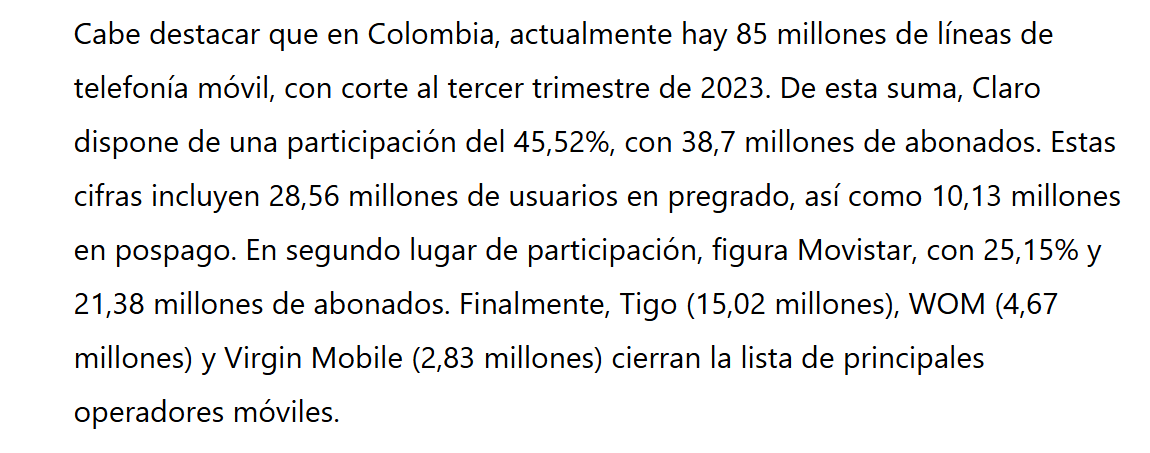
\includegraphics[width=0.9\textwidth]{../Images/MobilePhones/MobilePhoneMarket1.png}  
Referencia: \href{https://www.americaeconomia.com/negocios-e-industrias/hay-libre-competencia-en-el-mercado-de-telefonia-movil-de-colombia}{americaeconomia.com}
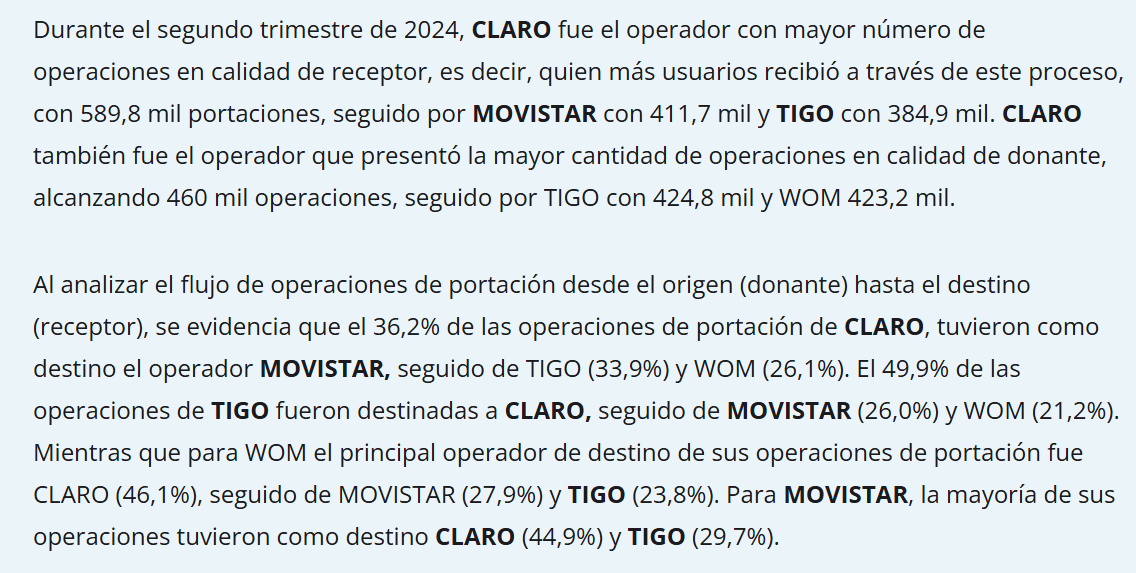
\includegraphics[width=0.9\textwidth]{../Images/MobilePhones/MobilePhoneMarket2.png} 
Referencia: \href{https://www.prensario.net/Colombia-Usuarios-solicitaron-174-millones-de-cambios-de-operador-movil-durante-el-segundo-trimestre-de-2024-47330.note.aspx}{prensario.net}
\end{center}

Asumí que los datos de la primera noticia (febrero de 2024) reflejan de manera válida el estado del mercado al cierre del primer trimestre de ese año.

\begin{enumerate}
\item Completá la tabla con el número total de usuarios por operador al final del primer trimestre de 2024:

\begin{tabular}{|c|c|c|c|c|c}
\hline
Claro & Movistar & Tigo & Wom & Otras \\
\hline
& & & & \\
\hline
\end{tabular}

\item Basándote en la información disponible, completá la tabla con el flujo de usuarios que cambiaron de un proveedor a otro durante el segundo trimestre de 2024. Si necesitás estimar valores ante la falta de datos explícitos, justificá detalladamente tu razonamiento.

\begin{tabular}{|c|c|c|c|c|c|}
\hline
& Claro & Movistar & Tigo & Wom & Otras \\
\hline
Claro & & & & & \\
\hline
Movistar & & & & & \\
\hline 
Tigo & & & & & \\
\hline 
Wom & & & & & \\
\hline
Otras & & & & & \\
\hline
\end{tabular}
\item Modelá la elección de proveedor de un usuario a lo largo del tiempo como un proceso markoviano. Especificá  el espacio de estados y estimá la matriz de transición correspondiente.
\item Transcurridos 2 años, ¿cuál es la participación de mercado (\textit{market share}) esperada para cada operador? Asumí que el tamaño total del mercado se mantiene constante (no entran ni salen usuarios del sistema).
\item Determiná la distribución de equilibrio del sistema. ¿Cuál es la participación de mercado esperada a largo plazo para cada proveedor? ¿Bajo qué hipótesis es válida esta conclusión?
\end{enumerate}
\item En clase analizamos un modelo de gestión de stock diario bajo una política fija $(n, N)$, con tiempo de entrega nulo ($L=0$) y demanda estocástica $i.i.d.$ Considerá ahora la extensión de este modelo ante un escenario estacional.

Asumí un año comercial de 364 días dividido en cuatro estaciones exactas de 91 días (verano, otoño, invierno, primavera) que se suceden cíclicamente. La demanda diaria $D_t$ es binaria y su distribución depende de la estación:
\begin{itemize}
    \item Verano / Invierno: $P(D_t = 2) = 0.8$ y $P(D_t = 1) = 0.2$
    \item Otoño / Primavera: $P(D_t = 2) = 0.3$ y $P(D_t = 1) = 0.7$
\end{itemize}

Formulá esta situación como un proceso markoviano con recompensa (MRP) resolviendo los siguientes puntos:

\begin{enumerate}
    \item Definí formalmente los estados del sistema. Explicá por qué registrar únicamente el nivel de inventario físico viola la propiedad de Markov y qué variable de estado debés incorporar para preservarla.
    
    \item Determin\'a las probabilidades de transición $P_{ss'}$ entre un estado genérico $s$ y su sucesor $s'$.
    
\item En clase definimos la recompensa inmediata en función de la demanda observada:
{\small
$$ r(X_t, D_t) = p \min(X_t, D_t) - h X_t - q \max(0, D_t - X_t) - K \mathbb{I}(X_t - D_t \leq n) $$
}donde $p$ es el precio, $h$ el costo de inventario, $q$ la penalidad por quiebre y $K$ el costo de orden. Dado que un MRP requiere una función de recompensa que dependa únicamente del estado, calculamos el valor esperado respecto a la distribuci\'on de la demanda: $r(s) = \mathbb{E}_D[r(s, D)]$. 

Considerando que ahora tu definición de estado $s$ es más amplia que el simple nivel de inventario físico, describí explícitamente cómo se calcula la recompensa en funci\'on de $s$ bajo la nueva formulación.
    
    \item Asumiendo que $N = 100$, ¿cuál es la cardinalidad del espacio de estados? 
    
    \item Para reducir la complejidad computacional del modelo, un consultor propone cambiar de un paso de tiempo diario a uno semanal. 
    \begin{itemize}
        \item ¿Cómo afectaría este cambio a la cardinalidad del espacio de estados?
        \item Desde una perspectiva comercial y logística, ¿qué impacto  tendría gobernar el inventario semanalmente en lugar de diariamente?
    \end{itemize}
\end{enumerate}

\end{enumerate}
\end{document}